\documentclass[11pt]{article}
\usepackage[T1]{fontenc}
\usepackage[utf8]{inputenc}
\usepackage{mathpazo}
\usepackage{courier}
\usepackage[margin=1.02in]{geometry}
\usepackage{amsmath,amssymb,amsthm,mathtools}
\usepackage{microtype}
\usepackage{needspace}
\usepackage{enumitem}
\usepackage{booktabs}
\usepackage{tikz}
\usetikzlibrary{arrows.meta,positioning,calc,decorations.pathreplacing}
\usepackage{xcolor}
\usepackage[numbers,sort&compress]{natbib}
\usepackage[colorlinks=true,linkcolor=blue!45!black,citecolor=blue!45!black,urlcolor=blue!45!black]{hyperref}
\usepackage[nameinlink,capitalise,noabbrev]{cleveref}
\newcommand{\doi}[1]{doi: \href{https://doi.org/#1}{\nolinkurl{#1}}}
\pdfinfoomitdate=1
\pdftrailerid{}
\pdfsuppressptexinfo=15
\pdfglyphtounicode{parenleftbig}{0028 FE01}
\pdfglyphtounicode{parenrightbig}{0029 FE01}
\pdfglyphtounicode{braceleftBigg}{007B FE04}
\pdfglyphtounicode{uniondisplay}{22C3 FE02}
\pdfglyphtounicode{hatwide}{02C6 FE01}
\pdfglyphtounicode{tildewide}{02DC FE01}
\pdfgentounicode=1
\hypersetup{pdftitle={A Polynomial-Time Algorithm for Three-Machine Unit-Job Scheduling},pdfauthor={OpenAI}}
\usepackage{caption}
\captionsetup{font=small,labelfont=bf}
\setlength{\emergencystretch}{2em}
\setlist[enumerate]{itemsep=3pt,topsep=5pt}
\setlist[itemize]{itemsep=3pt,topsep=5pt}
\numberwithin{equation}{section}
\newtheorem{theorem}{Theorem}[section]
\newtheorem{lemma}[theorem]{Lemma}
\newtheorem{proposition}[theorem]{Proposition}
\newtheorem{corollary}[theorem]{Corollary}
\theoremstyle{definition}
\newtheorem{definition}[theorem]{Definition}
\theoremstyle{remark}
\newtheorem{remark}[theorem]{Remark}
\newcommand{\F}{\mathcal F}
\newcommand{\K}{\mathbf K}
\newcommand{\Qual}{\mathcal Q}
\newcommand{\key}{\operatorname{key}}
\newcommand{\rk}{\lambda}
\newcommand{\wP}[1]{\widehat P_{#1}}
\newcommand{\wD}[1]{\widehat D_{#1}}
\newcommand{\A}{\mathsf A}
\newcommand{\dotcup}{\mathbin{\dot\cup}}
\newcommand{\poly}{\operatorname{poly}}
\newcommand{\YES}{\mathsf{YES}}
\newcommand{\NO}{\mathsf{NO}}
\newcommand{\low}{\mathsf{low}}
\newcommand{\high}{\mathsf{high}}
\newcommand{\same}{\mathsf{same}}
\newcommand{\switch}{\mathsf{switch}}

\title{A Polynomial-Time Algorithm for Three-Machine\\
Unit-Job Scheduling}
\author{OpenAI}
\date{September 24, 2026}

\begin{document}
\maketitle
\begin{abstract}
We give a uniform deterministic polynomial-time algorithm for scheduling
unit-length jobs with arbitrary precedence constraints on three identical
parallel machines. The algorithm constructs a schedule of minimum makespan
and decides exactly whether all jobs can finish by a specified deadline.
The proof reorganizes feasible schedules
into intervals whose job sets have descriptions of bounded size.
A dynamic program searches a family containing polynomially many such
descriptions. Global boundary conditions and simplification of inherited
information keep the descriptions bounded throughout the decomposition.
\end{abstract}

\section{Introduction}\label{sec:introduction}

A precedence-constrained schedule must respect two kinds of restrictions:
jobs related by precedence must run in order, while unrelated jobs compete
for the available machines. Even when every job takes one unit of time, the
interaction between these restrictions is subtle. The two-processor case
was treated by Fujii, Kasami, and Ninomiya
\citep{FujiiKasamiNinomiya1969,FujiiKasamiNinomiya1971Erratum}, and
Coffman and Graham gave an optimal list-scheduling algorithm
\citep{CG1972}. Allowing the number of machines to be part of the input
yields an NP-complete problem \citep[Theorem~1]{Ullman1975}.
The fixed-three decision problem appears as OPEN8 in Appendix~A13 of
Garey and Johnson \citep{GJ1979} and has remained a central complexity
question in scheduling \citep{NSW2025}.

We consider the following precise decision problem. The input is an
explicitly listed directed acyclic graph \(G=(V,E)\), with
\(V=\{1,\ldots,n\}\), and an integer \(T\) satisfying \(1\le T\le n\).
Every vertex is a nonpreemptive job of processing time one. The question
is whether there is a function
\[
 \tau:V\longrightarrow\{1,\ldots,T\}
\]
such that each value is taken at most three times and
\(\tau(u)<\tau(v)\) for every \((u,v)\in E\).
There are no release dates, communication delays, eligibility restrictions,
or additional resources.
Slot \(t\) means execution during \([t-1,t)\), and the makespan is
the last completion time. Allowing nonnegative real start times would
not improve the optimum: fix the machine assignment and within-machine
order of a feasible schedule. The graph augmented by machine-order arcs
is acyclic, as witnessed by the original schedule. In a topological order
of this graph, set each start time to the maximum of zero and its
predecessors' completion times. Induction gives integer start times,
and no completion time increases.
The standard notation for the problem is
\(P3\mid\mathrm{prec},p_j=1\mid C_{\max}\)
\citep{GrahamLawlerLenstraRinnooyKan1979}.

\begin{samepage}
\begin{theorem}\label{thm:main}
Let an explicitly listed finite directed acyclic graph specify the
precedence constraints on \(n\ge1\) nonpreemptive unit-length jobs
on three identical machines. There is a uniform deterministic algorithm
that constructs a feasible schedule of minimum makespan.
Given also an integer deadline \(1\le T\le n\), it decides feasibility
exactly and returns a schedule whenever the answer is affirmative.
Both tasks can be performed in
\(O((L+2)^{150020})\) steps on a deterministic multitape Turing machine,
where \(L\) is the total binary input length.
\end{theorem}
\end{samepage}

The theorem resolves the polynomial-time side of this three-machine
complexity question. Its scope is the explicit model just stated.
The polynomial supplied by the proof has a very large constant exponent;
no practical running-time claim is made.

\paragraph{Prior work and the point of departure.}
Structural restrictions on precedence yield important intermediate
results. Garey, Johnson, Tarjan, and Yannakakis gave a linear-time
algorithm on three processors for opposing forests, which are disjoint
unions of an in-forest and an out-forest
\citep[Section~4]{GareyJohnsonTarjanYannakakis1983}.
Dolev and Warmuth obtained a running time
\(O(n^{h(m-1)+1})\) when the precedence graph has height \(h\), measured
in arcs, and at most \(m\) processors are available in each slot
\citep[Theorem~3]{DW1984}. The available number may vary over time.
This is polynomial when both \(h\) and \(m\) are fixed.
Their normalized optimal schedules, called zero-adjusted, have a slot
whose at most \(m-1\) jobs with successors determine the prefix and the
remaining subproblem, the latter up to isomorphism. When the graph has positive
height, both recursive pieces have smaller height
\citep[Theorem~2]{DW1984}.

Nederlof, Swennenhuis, and Węgrzycki developed this structural approach
into an exact algorithm with running
time \((1+n/m)^{O(\sqrt{nm})}\) for \(n\) jobs on \(m\) machines, hence
\(2^{O(\sqrt n\log n)}\) for three machines
\citep[Theorem~1.1]{NSW2025}.
Their decomposition at selected slots and memoization of subproblems
described by source and sink sets already control the number of
subproblems despite potentially linear recursion depth
\citep[Sections~5--6]{NSW2025}. Their proper-decomposition
theorem assumes at most \(m\) sources
\citep[Definition~1 and Theorem~3.1]{NSW2025}; their full algorithm
handles arbitrary precedence graphs. The marked intervals below build on
this decomposition viewpoint. We prove the required separator statements
and bound the size of each global interval description directly; the
polynomial bound does not follow by specializing their subexponential bound.

Approximation algorithms also revealed useful recursive structure.
For fixed machine count and fixed \(\varepsilon>0\), Levey and Rothvoß
obtained a \((1+\varepsilon)\)-approximation using linear programming
(LP) hierarchies
\citep{LeveyRothvoss2016}; Garg improved the running time to
quasipolynomial \citep{Garg2018}. Li replaced LP conditioning by
combinatorial guesses and obtained the bound
\(n^{O((m^4/\varepsilon^3)(\log\log n)^3)}\) \citep{Li2021}.
Das and Wiese later gave a simpler combinatorial quasipolynomial-time
approximation scheme \citep{DasWiese2022}.
These works give a related perspective on the recursive structure of
nearly optimal schedules. The exact separator and global-description
statements used here are established separately.

\paragraph{Why a finite search can suffice.}
After adding isolated jobs, we may assume that every slot contains three
jobs. If selected slots are removed from a feasible schedule, the remaining
open gaps can be scheduled independently: reordering the jobs of one gap
does not change their temporal relation to any exterior job. This suggests
a recursive search whose subproblems are the sets of jobs in those gaps.
The obstacle is their number. Naming a gap by its two boundary triples
does not by itself determine its job set, and repeatedly intersecting
descriptions inherited from its ancestors can require an unbounded formula.

We prove that every feasible instance has a recursive decomposition in
which each gap is described \emph{globally}, as a subset of all jobs, by a
Boolean formula of bounded size. The permitted tests are precedence to or
from a triple of jobs, membership in that triple, and rank thresholds in
a fixed linear extension or its reverse. The bound is independent of the
depth of the decomposition. There are therefore only polynomially many
sets that the algorithm must consider. Compatible selected triples connect
smaller accepted gap sets, and their concatenation gives the schedule.

The structural proof chooses lexicographically minimal schedules only as
existence witnesses; the algorithm enumerates the descriptions instead of
computing those witnesses. Fix a priority order extending precedence,
and call its current initial segment low and the remaining jobs high.
A selected slot separates this cutoff when every earlier high job is a
precedence predecessor of a job in that slot, and every later low job is
a precedence successor of one. In a normalized interval, we promote
jobs one at a time from high to low and move a separator forward. Each pair
of successive selected slots separates one common cutoff: each low job
in the intervening gap has a predecessor in its left slot, and each high
job has a successor in its right slot.

The two sides of a center slot are treated by the same construction:
for one side we reverse both time and precedence. To describe a gap
without remembering all its ancestors, we maintain a short list of sets
closed under taking successors in the current direction. A boundary slot limits the number of new list entries that can
survive. A global boundary condition excludes distant jobs, while an
exchange condition keeps that control valid after later reorderings.
At a change of direction, a paired form of the inherited entries lets us
replace their history by a bounded formula. The distinction between
agreement inside a known interval and a description valid on all jobs is
what makes this last step necessary.

\paragraph{Organization.}
\Cref{sec:preliminaries,sec:algorithm} specify a finite description family
and the uniform algorithm. \Cref{sec:separators} supplies common cutoffs,
and \Cref{sec:construction} uses them to form smaller child intervals.
\Cref{sec:lists} bounds inherited predicate information;
\Cref{sec:boundary} proves the global boundary invariants.
\Cref{sec:descriptions} describes whole intervals and marked
splits by bounded formulas, completing the hierarchy proof.
\Cref{sec:complexity} gives the explicit running-time bound.

\section{Full schedules, frames, and descriptions}\label{sec:preliminaries}

We write \(x\prec y\) if there is a directed path of positive length
from \(x\) to \(y\). Transitive reachability can be computed in polynomial
time. All restrictions of the precedence order below mean restrictions of
this transitive order, including when a path in the original graph uses
vertices outside the restricted set.

\subsection{Padding and interval reorderings}

If \(n>3T\), reject. Otherwise add \(3T-n\) isolated jobs and let \(J\)
be the resulting set, with \(N=|J|=3T\).
A \emph{full schedule} of a set \(W\subseteq J\) is an ordered sequence
of antichain triples partitioning \(W\), respecting \(\prec\).
Its length is necessarily \(|W|/3\). The empty set has the empty full
schedule.

\begin{lemma}\label{lem:padding}
The original deadline is feasible if and only if \(J\) has a full schedule.
The padded instance has polynomial size in the stated input encoding.
\end{lemma}
\begin{proof}
A schedule of the original jobs leaves exactly \(3T-n\) vacant positions
among the three machines and \(T\) slots. Fill them with the isolated jobs.
Conversely, delete the isolated jobs from a full schedule.
Since \(T\le n\) and the vertices are explicitly listed, \(N=3T\le3n\)
is polynomially bounded.
\end{proof}

A schedule's slots will also denote their job triples. An \emph{open
interval} \((a,b)\) consists of all slots strictly between two boundary
slots; we use the same symbol \(W\) for that interval's job set.
Virtual boundaries before the first and after the last slot are allowed.

\begin{lemma}\label{lem:reorder}
Replacing the schedule inside an open interval by any full schedule of
its job set preserves feasibility of the complete schedule.
\end{lemma}
\begin{proof}
All exterior jobs are either before the entire interval or after it.
Their order relative to every interior job is unchanged. Interior
precedences hold by the assumed feasibility of the replacement.
\end{proof}

\subsection{The two frames}

Fix a linear extension of the order on \(J\), with rank
\(\rk:J\to\{1,\ldots,N\}\). A deterministic choice is obtained by
successively removing a minimal job, breaking ties by its identifier.
We also use the reversed order, reversed time, and reversed linear
extension. These are our two \emph{frames}. The two ranks of a job sum
to \(N+1\). Unless a frame is specified otherwise, all time comparisons,
precedence relations, and ranks in an argument belong to its working frame.

For an actual slot \(a\), identified with its job triple, define global cones
\[
 D_a=\{x\in J:\exists y\in a,\ y\prec x\},
 \qquad
 P_a=\{x\in J:\exists y\in a,\ x\prec y\},
 \qquad
 \wD a=D_a\cup a,\quad \wP a=P_a\cup a .
\]
At the left sentinel take \(D_a=\wD a=J\) and
\(P_a=\wP a=\varnothing\). At the right sentinel use the opposite
convention. Reversal exchanges \(D\) and \(P\), and exchanges their
weak versions. In a fixed frame the \(D\)-cones and weak \(D\)-cones are
upward closed, whereas the \(P\)-cones and weak \(P\)-cones are downward
closed.

Cone membership always concerns the whole poset \(J\), even when a formula
is evaluated on an interval. A job that is temporally earlier than a block
need not be a predecessor of that block.

\subsection{A fixed finite family}

Let \(\F\) be the family of subsets of \(J\) described by Boolean formulas
with at most \(K=10000\) leaves. Leaves are the following atomic tests or
their negations:
\begin{itemize}
 \item true and false;
 \item rank thresholds \(\rk\le k\) and \(\rk\ge k\), with
 \(0\le k\le N+1\), in either frame;
 \item membership in a triple of jobs, or in any of its four cones
 \(P,D,\widehat P,\widehat D\), in either frame.
\end{itemize}
Internal nodes are binary conjunctions and disjunctions. Negating a formula
does not increase its number of leaves: apply De Morgan's laws and push
negations to the leaves. Sentinel tests are constants.
We distinguish a \emph{global description} \(W=F\), with \(F\in\F\),
from a \emph{relative description} \(L=W\cap F\).

\begin{lemma}\label{lem:family}
The family \(\F\) can be generated deterministically in polynomial time
and represented by \(N\)-bit vectors.
\end{lemma}
\begin{proof}
There are \(O(N^3)\) atomic tests. The number of binary tree shapes and
connective assignments with at most \(K\) leaves is a constant depending
only on \(K\). Labelling the leaves therefore gives \(O(N^{3K})\)
formulas, with a constant implicit factor. Compute their truth sets after
precomputing reachability, then deduplicate by comparing the bit vectors
pairwise. This is a deterministic finite procedure with polynomial cost.
\end{proof}

\section{The algorithm and its structural certificate}\label{sec:algorithm}

The algorithm accepts or rejects each \(W\in\F\), in increasing order
of cardinality. Write \(\A(W)\) for its acceptance value, and regard
\(\A(U)\) as false when \(U\notin\F\).
Set \(\A(\varnothing)\) to true, and reject sets whose sizes are not
divisible by three.

For each remaining nonempty \(W\), form states
\[
 (L,Z,R),\qquad W=L\dotcup Z\dotcup R,
\]
where \(Z\) is an antichain triple and \(L=W\cap F\) for some \(F\in\F\).
Keep a state only if the displayed order of its three parts is
\emph{compatible}: no job in a later part precedes a job in an earlier
part. This test uses the transitive order on \(J\).
Declare the state initial when \(\A(L)\) is true and final when
\(\A(R)\) is true. Add an edge
\[
 (L,Z,R)\longrightarrow(L',Z',R')
\]
exactly when
\begin{equation}
 L\cup Z\subseteq L',
 \qquad
 \A\bigl(L'\setminus(L\cup Z)\bigr)=\mathrm{true}.
 \label{eq:transition}
\end{equation}
All acceptance values consulted concern smaller sets.
Set \(\A(W)\) to true if an initial state reaches a final state,
allowing a path consisting of a single state.
Return \(\YES\) precisely when \(\A(J)\) is true.

\begin{proposition}\label{prop:algorithm}
This is a uniform deterministic polynomial-time algorithm. Every set it
accepts has a full schedule, which the algorithm can explicitly return.
With \(K=10000\), its deadline decision and schedule construction take
\(O((L+2)^{150020})\) deterministic multitape steps.
\end{proposition}
\begin{proof}
For soundness, consider a path with triples \(Z_1,\ldots,Z_k\) and
left sets \(L_1,\ldots,L_k\). Put
\[
 A_0=L_1,\qquad
 A_i=L_{i+1}\setminus(L_i\cup Z_i)\ (1\le i<k),\qquad
 A_k=R_k.
\]
The inclusions in \eqref{eq:transition} give the ordered disjoint partition
\begin{equation}
 W=A_0\dotcup Z_1\dotcup A_1\dotcup\cdots
       \dotcup Z_k\dotcup A_k.
 \label{eq:partition}
\end{equation}
Every \(A_i\) is smaller than \(W\) and was already accepted. By induction
it has a full schedule. Every two distinct pieces in \eqref{eq:partition}
are separated by a selected state, with the earlier piece in its left
part or triple and the later piece in its triple or right part.
Compatibility of that state excludes a backward precedence between
the pieces. Concatenating their schedules with the selected triples is
therefore a full schedule of \(W\).

To produce that schedule, record a predecessor whenever a state is
first reached, with initial states distinguished as roots. Trace back
from a reached final state and use the partition \eqref{eq:partition}.
Along every transition \(|L|\) increases by at least three, so an
accepting path has at most \(N/3\) triples. Retrieve the already stored
schedules of its smaller gap sets and concatenate them with those
triples. Store this one explicit schedule for \(W\), avoiding any
repeated recursive expansion.

There are only polynomially many formula instances, sets, states,
and state pairs because the leaf allowance $K$ is fixed. Sequential scans
of their bit-vector records therefore give a uniform polynomial-time
implementation. \Cref{sec:complexity} gives the explicit multitape
accounting, including the scans and copying needed for reconstruction,
and proves the stated exponent.
\end{proof}

The completeness certificate uses only intervals, their marked triples,
and descriptions; it imposes no bound on the number of levels.

\Needspace{3\baselineskip}
\begin{definition}\label{def:hierarchy}
A \emph{bounded-description hierarchy} for a feasible \(J\) has the whole
schedule as its root interval. At a nonempty node \(W\), one may first
replace its schedule by a full schedule of the same job set. One then
marks at least one actual slot; the nonempty open gaps between successive
marks and the two boundaries become its children. Different children may
be developed with separate copies of their witnessing exterior schedules.
The following descriptions are required:
\begin{enumerate}[label=(\roman*)]
 \item every node job set belongs to \(\F\);
 \item for every marked triple, its earlier jobs within the node have a
 relative description \(W\cap F\), with \(F\in\F\), in original time.
\end{enumerate}
\end{definition}

\begin{lemma}\label{lem:hierarchy-dp}
If a feasible \(J\) has a bounded-description hierarchy, the algorithm
accepts \(J\).
\end{lemma}
\begin{proof}
Induct on node size. Its marks give compatible states in chronological
order by property (ii). Their end gaps and transition gaps are empty
or are its children, belong to \(\F\), and are strictly smaller because
there is an actual mark. They have already been accepted by induction.
The states consequently give an initial-to-final path.
The root belongs to \(\F\) because its predicate is true.
\end{proof}

We prove the following structural assertion in
\Cref{sec:separators,sec:construction,sec:lists,sec:boundary,sec:descriptions}.
The considerably larger allowance \(K=10000\) avoids dependence on tight
constant bookkeeping.

\begin{theorem}\label{thm:structure}
Every feasible full three-machine schedule has a bounded-description
hierarchy. In fact, the global node predicates and relative split
predicates needed in the hierarchy have fewer than \(500\) leaves.
\end{theorem}

\begin{proof}[Proof of \Cref{thm:main}, assuming \Cref{thm:structure}]
Apply \Cref{lem:padding,prop:algorithm,lem:hierarchy-dp,thm:structure}.
The algorithm is sound on every enumerated set and complete at \(J\).
For makespan minimization, test all deadlines \(1,\ldots,n\) and take
the smallest feasible one. A topological ordering gives a feasible
schedule of length at most \(n\), so this search succeeds.
Return the stored full schedule for its padded instance and delete the
isolated padding jobs. Assign the at most three remaining jobs in each
slot to distinct machines. The schedule has optimum makespan by the
choice of deadline. The bound in \Cref{prop:algorithm} already allows
all these deadline trials.
\end{proof}

\section{Separators with a shared cutoff}\label{sec:separators}

Decomposing a normalized schedule at selected slots is a central device
in Dolev--Warmuth \citep[Theorem~2]{DW1984} and in the proper-decomposition
construction of Nederlof, Swennenhuis, and Węgrzycki
\citep[Section~3]{NSW2025}. Here we prove the shared-cutoff form needed
for the interval construction: successive boundaries must separate the
same ideal of low-priority jobs. The global-list invariants in later
sections control these descriptions inside descendant intervals.

This section concerns one fixed frame and a domain consisting of a
contiguous interval of a feasible schedule. A set is an \emph{ideal}
in the domain if it contains every domain predecessor of each of its
members. Its complement in the domain is an upset.

\begin{definition}\label{def:separator}
Given an ideal \(S\) of low jobs in a domain, a slot \(z\) is a
\emph{separator at cutoff \(S\)} if
\begin{enumerate}[label=(\alph*)]
 \item every domain job before \(z\) that is outside \(S\) belongs to \(P_z\);
 \item every domain job after \(z\) that belongs to \(S\) belongs to \(D_z\).
\end{enumerate}
The other domain jobs are called high. A left boundary outside the domain
is also a separator when all low domain jobs descend from it; there are
then no domain jobs before that boundary.
\end{definition}

An actual separator has a useful description of its earlier jobs. For
a global set \(H\subseteq J\), put
\begin{equation}
 B_z(H)=P_z\cup\bigl(H\setminus\wD z\bigr).
 \label{eq:B-definition}
\end{equation}

\begin{lemma}\label{lem:separator-description}
If \(z\) is an actual separator for a domain \(U\) at cutoff \(S\),
and \(H\cap U=S\), then \(B_z(H)\cap U\) is exactly the set of
domain jobs strictly earlier than \(z\). Reversing order and time,
and exchanging low with high, preserves the separator property.
\end{lemma}
\begin{proof}
Every job in \(P_z\) is strictly earlier than \(z\). An earlier low
job is outside \(\wD z\). A low job at \(z\) belongs to \(\wD z\),
and a later low job belongs to \(D_z\) by separation. Finally, every
earlier high job belongs to \(P_z\). These observations give both
inclusions. Reversal exchanges the two conditions in
\Cref{def:separator}.
\end{proof}

\subsection{Lexicographic normalization}

A \emph{priority order} is a total order of the domain extending
precedence. Read a full schedule chronologically, with each triple sorted
by priority. Among the finitely many feasible full schedules of the
domain, choose one whose resulting sequence of priority indices is
lexicographically least. Call it \emph{normalized} for that priority.
This is an existence choice, not an operation of the decision algorithm.

\begin{lemma}\label{lem:lex-prefix}
In a normalized schedule, a feasible exchange that puts a better-priority
job into an earlier slot is impossible. More generally, fix a slot \(r\).
After any feasible reordering confined strictly after \(r\), a feasible
exchange of a job at \(r\) with a better-priority job at a later slot
is still impossible.
\end{lemma}
\begin{proof}
Replacing one member of a sorted triple by a better-priority job
lexicographically improves that triple. In the second assertion, the
schedule through \(r\) is unchanged by the intervening reordering.
The proposed exchange would therefore first change the normalized
sequence at \(r\), and improve it there. The resulting full schedule
would contradict minimality, regardless of what happens later.
\end{proof}

\begin{lemma}[Shared-cutoff walk]\label{lem:shared}
Fix a normalized full schedule of a domain and let \(S\) and \(S^+\)
be consecutive priority prefixes, differing by the promotion of one job
from high to low. Suppose \(s\) is a separator at cutoff \(S\),
either inside the domain or at its exterior left boundary.
Then there is a separator \(t\ge s\), found by advancing only to
domain slots on the right, that separates both \(S\) and \(S^+\).
If the priority order is specified on a larger job set and the promoted
job is outside the domain, one may take \(t=s\).
\end{lemma}
\begin{proof}
\textbf{One advance at a fixed cutoff.}
Keep the normalized schedule and its priority order fixed. Let \(L\)
be a prefix of that priority order, and suppose the current position
\(s\) satisfies the earlier-high condition for \(L\).
If a later low job does not descend from \(s\), choose the earliest
slot \(t>s\) containing such a job, and choose one of them, \(x\).
Every domain predecessor of \(x\) lies strictly before \(s\).
Indeed, that predecessor is low because \(L\) is an ideal.
A predecessor at \(s\) would force \(x\in D_s\). A predecessor
strictly between \(s\) and \(t\) would descend from \(s\), by the
earliest choice of \(t\), and again force \(x\in D_s\).

Let \(y\) be a high domain job at a slot \(r\) with \(s\le r<t\).
If \(y\) had no domain successor at or before \(t\), exchanging
\(x\) and \(y\) would be feasible: all predecessors of \(x\) are
before \(s\), and delaying \(y\) would violate no successor
constraint. Moving \(x\) earlier and \(y\) later preserves their
other precedence constraints. Since \(L\) is a priority prefix,
\(x\) has better priority than \(y\), contradicting
\Cref{lem:lex-prefix}. Thus \(y\) has a successor by \(t\).
The successor is high, since the high set is an upset. If it is
strictly before \(t\), repeat the argument. Strictly increasing
times give a chain from \(y\) to a high job at \(t\).

When \(s\) is internal, every earlier high job has a descendant
at \(s\) by the earlier-high condition. That descendant is high,
and the preceding tracing extends the chain to \(t\).
When \(s\) is the exterior left boundary, there are no earlier
domain jobs. Hence \(t\) satisfies the earlier-high condition.
We may advance to \(t\) and repeat until there is no later low
exception. There are finitely many slots, and every advance is
strict, so the final position also satisfies the later-low condition.
Throughout this walk the normalized schedule itself stays fixed;
only the selected separator position changes.

\smallskip\noindent\textbf{Adding one low job.}
Apply this procedure with \(L=S^+\), starting at the given
separator for \(S\). The earlier-high condition for \(S^+\)
holds initially because its high set is smaller. If no advance is
needed, the same position separates both cutoffs.

Otherwise the first exception is the single promoted job: every
later job already low at \(S\) descends from the starting position.
At the first target, the promoted job lies in that target slot,
so it introduces no earlier high job for the old cutoff \(S\).
Thus the earlier-high condition holds there for both cutoffs.

In every subsequent advance, the exception is old-low: the promoted
job stays at the first target, at or before the current position.
An old-low exception has better priority than every old-high job.
The same exchange and successor tracing therefore propagates the
earlier-high condition for \(S\) as well as for \(S^+\).
At the final position, the later-low condition for \(S^+\) also
implies the later-low condition for \(S\), since \(S\subseteq S^+\).
The final position separates both cutoffs.

If the promoted job is outside the domain, the two restricted
prefixes coincide, so the original position already separates both.
\end{proof}

\begin{corollary}\label{cor:any-ideal}
Every ideal of a nonempty set with a full schedule has an actual
separator in some full schedule of that set.
\end{corollary}
\begin{proof}
Prioritize the ideal before its complement, using a linear extension
inside each. Normalize. The first actual slot separates the empty
prefix. Promote the jobs of the ideal one by one and use
\Cref{lem:shared}. The final position is an actual separator for
the ideal.
\end{proof}

The shared cutoff, rather than merely the existence of separate
separators, will be used for a gap: its low jobs descend from its
left endpoint, while its high jobs precede its right endpoint.
Keeping the final position of each promotion is important. Intermediate
positions assist the proof but need not become marks.

\section{The interval construction and its invariants}\label{sec:construction}

We now construct the hierarchy from a feasible full schedule of \(J\).
Each node has a \emph{tag}, one of the two frames, and a witnessing
complete schedule. Descending to a child changes only the jobs inside
that child; its boundary triples and exterior schedule remain fixed.
Branches can retain separate witnesses, as allowed in
\Cref{def:hierarchy}.

\subsection{Global lists and boundary conditions}

In the tag frame of a node \(W=(a,b)\), attach an ordered list
\(\K=(K_1,\ldots,K_\ell)\) of global upsets.
Define the global qualifier set and the local old-high set by
\[
 \Qual(\K)=\bigcup_{i=1}^{\ell}K_i,
 \qquad O=W\cap\Qual(\K).
\]
For every globally qualifying job \(x\), set
\begin{equation}
 \key_{\K}(x)=
 \left(\max\{i:x\in K_i\},\,\rk(x)\right),
 \label{eq:key}
\end{equation}
with lexicographic comparison. Entries may overlap. Their largest index,
not their smallest one, is used.
Because each entry is an upset, \(x\prec y\) with \(x\) qualifying
implies that \(y\) qualifies and
\(\key_{\K}(x)<\key_{\K}(y)\).

We maintain the following three invariants in the node's tag frame.
\begin{enumerate}[label=\textup{(I\arabic*)},ref=I\arabic*]
 \item\label{inv:cones}
 \(O\subseteq P_b\), and \(W\setminus O\subseteq D_a\).
 \item\label{inv:past}
 Every global qualifier scheduled at or before \(a\) belongs to
 \(\wP a\).
 \item\label{inv:swap}
 After \emph{any} feasible reordering of \(W\) in its existing slots,
 there is no feasible direct exchange between
 \(x\in W\setminus D_a\) and a qualifying job \(y\) at \(a\) when
 \(\key_{\K}(x)<\key_{\K}(y)\).
\end{enumerate}
Invariant~\ref{inv:cones} controls the jobs inside the interval;
Invariant~\ref{inv:past} controls qualifiers outside its left boundary,
and Invariant~\ref{inv:swap} makes that control persist after later
reorderings.

The exchange in Invariant~\ref{inv:swap} is tested for feasibility in
the complete schedule. The hypothetical exchanged schedule need not
preserve any decomposition or any of the list invariants.
The key of \(x\) is defined because Invariant~\ref{inv:cones} implies
\(W\setminus D_a\subseteq O\). A sentinel has no boundary jobs, so
the corresponding exchange condition is vacuous.

Lexicographic minimality within an interval controls exchanges of its
interior jobs; it gives no such control over exchanges with an exterior
boundary job. Invariant~\ref{inv:swap} supplies the latter control.
Suppose a qualifying job \(x\in W\setminus D_a\) has all its
predecessors strictly before \(a\), and its key is smaller than
that of a qualifying \(y\in a\). If \(y\) had no successor at or
before the slot of \(x\), their exchange would be feasible.
Invariant~\ref{inv:swap} therefore forces such a successor.
The proof in \Cref{sec:boundary} uses this first successor to
connect exterior qualifiers to the local separator walk.

All predicates are frozen global subsets of \(J\) once constructed.
In particular, a cone used in an old predicate continues to refer to
its fixed triple of jobs; it is not redefined after later reorderings.
We shall prove, simultaneously with the three invariants, that each
pruned list has at most five entries and each entry has fewer than
40 leaves.

At the root, use the original frame, the two sentinels, and the one-entry
list \((J)\). Invariant~\ref{inv:cones} follows from the sentinel cones,
and Invariants~\ref{inv:past} and~\ref{inv:swap} are vacuous.

\subsection{A center and two open sides}

In either working frame, let \(a,b\) now mean the left and right
boundaries of \(W\) in that frame, and write
\[
 X=W\setminus D_a,\qquad Y=W\setminus P_b.
\]
Invariant~\ref{inv:cones} gives
\begin{equation}
 W\subseteq D_a\cup P_b,\qquad X\subseteq P_b,\qquad Y\subseteq D_a.
 \label{eq:cover}
\end{equation}
This cover is unchanged by reversal: the two boundary cones exchange
roles. In either frame \(X\) is an ideal in \(W\), and \(Y\) an
upset. The list, \(O\), and the other two invariants are used in their
stated form only in the tag frame.

In the tag frame choose an actual center \(v\) separating
the ideal \(W\cap P_b\), using \Cref{cor:any-ideal} and, if needed,
reordering \(W\). Mark \(v\). At the root use the last slot as
center; it separates the ideal \(J\).
The center triple and the job sets on its two sides are now fixed.

Treat each side as an open prefix \(E=(a,v)\), in the frame that
makes it a prefix. Call that side \(\same\) if its working frame is
the node's tag and \(\switch\) otherwise. Recompute all boundary
notation in that working frame. The center is a separator at cutoff
\begin{equation}
 S_*=
 \begin{cases}
 W\cap P_b,&\same,\\
 X=W\setminus D_a,&\switch.
 \end{cases}
 \label{eq:center-cutoff}
\end{equation}
Indeed the second formula is the complement of the original center-low
set after reversing order and time, so
\Cref{lem:separator-description} applies.

Use the following priority orders on \(W\), and the following nested
low cutoffs.
\begin{description}[style=nextline,leftmargin=1.5em]
 \item[Same direction.]
 Begin with \(S_0=(W\setminus O)\cap P_b\).
 Order \(S_0\) first by increasing rank, then \(O\) by increasing
 \(\key_{\K}\), and then \(Y\) by increasing rank.
 Promote the jobs of \(O\) in that key order.
 \item[Switched direction.]
 Begin with \(S_0=\varnothing\).
 Order \(X\) first and \(W\cap D_a\) second, each by increasing
 rank in the switched frame.
 Promote the jobs of \(X\) in that order.
\end{description}
These are total orders extending precedence.
For the same case, \(S_0\) is an ideal, \(Y\) is an upset,
and the key order on the middle group extends precedence.
The groups partition \(W\) since \(O\subseteq P_b\).
For the switch case use idealness of \(X\).
Every cutoff lies in \(P_b\) on \(W\), by \eqref{eq:cover},
and the initial low set lies in \(D_a\).

Normalize the open side \(E\) using the restriction of its priority
order to \(E\). This can be done independently on the two sides
before constructing children. It preserves feasibility by
\Cref{lem:reorder} and preserves the center separator, since neither
side's job set changes.
The resulting sequence of low subsets of \(W\) is
\[
 S_0,S_1,\ldots,S_q=S_* .
\]
Some promoted jobs may lie outside \(E\).
Starting at its exterior left boundary \(s_0=a\), use
\Cref{lem:shared} for every promotion, taking \(s_i\) to be the
\emph{final} position of that promotion. Thus
\begin{equation}
 a=s_0\le s_1\le\cdots\le s_q<s_{q+1}=v.
 \label{eq:positions}
\end{equation}
The starting boundary is a separator on \(E\) because
\(S_0\cap E\subseteq D_a\).
For each \(i<q\), both \(s_i,s_{i+1}\) separate the cutoff \(S_i\)
on \(E\). The same assertion for \(i=q\) uses the center separator
at \(v\).

Mark the distinct actual walk positions in \(E\), in addition to \(v\).
For each strict step \(s_i<s_{i+1}\), use
\begin{equation}
 a'=s_i,\qquad b'=s_{i+1},\qquad S=S_i
 \label{eq:edge-data}
\end{equation}
as its edge data; Figure~\ref{fig:shared-cutoff} shows one such step.
Removing repetitions from \eqref{eq:positions}
does not create an unassigned gap: consecutive distinct positions
are exactly the endpoints of one of these strict steps.
If the gap \(W'=(a',b')\) is nonempty, make it a child and tag it
with this working frame.

\begin{lemma}\label{lem:edge-labels}
At every child edge, \(b'\) is an actual triple in \(W\), while
\(a'\) is either \(a\) or an actual triple of \(E\). On its child,
\begin{equation}
 W'\cap S\subseteq D_{a'}\cap P_b,
 \qquad
 W'\setminus S\subseteq P_{b'}.
 \label{eq:edge-labels}
\end{equation}
Every child excludes the center and is strictly smaller than its parent.
The root has no nonempty switched child.
\end{lemma}
\begin{proof}
The shared cutoff at \(a',b'\) gives the two required separator
implications on the open side. All cutoffs lie in \(P_b\) on \(W\).
The remaining assertions follow from the positions of the marks,
and from the root's last-slot center.
\end{proof}

\begin{figure}[t]
\centering
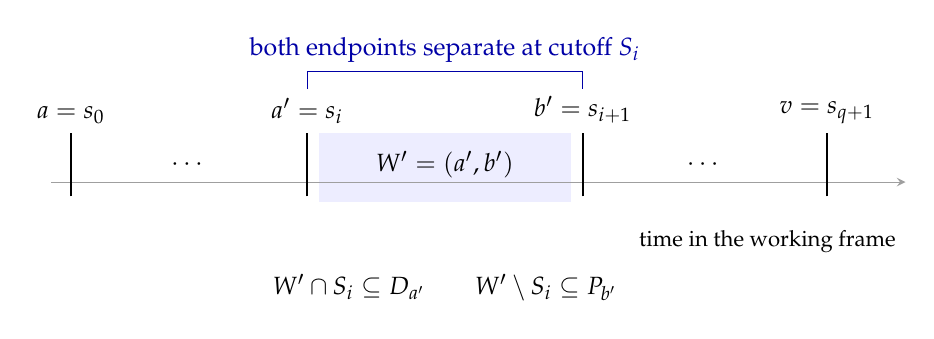
\begin{tikzpicture}[x=1cm,y=1cm,font=\small,>=stealth]
  \fill[blue!7] (3.15,-.25) rectangle (6.35,.62);
  \draw[->,gray!75] (-.25,0) -- (10.6,0);
  \node[anchor=east,font=\footnotesize] at (10.6,-.75)
    {time in the working frame};
  \foreach \x in {0,3,6.5,9.6}
    {\draw[thick] (\x,-.18) -- (\x,.62);}
  \node[above] at (0,.62) {$a=s_0$};
  \node[above] at (3,.62) {$a'=s_i$};
  \node[above] at (6.5,.62) {$b'=s_{i+1}$};
  \node[above] at (9.6,.62) {$v=s_{q+1}$};
  \node at (4.75,.22) {$W'=(a',b')$};
  \node at (1.5,.22) {$\cdots$};
  \node at (8.05,.22) {$\cdots$};
  \draw[blue!65!black] (3,1.18) -- (3,1.4) -- (6.5,1.4) -- (6.5,1.18);
  \node[above,text=blue!65!black] at (4.75,1.4)
    {both endpoints separate at cutoff $S_i$};
  \node[anchor=north,align=center] at (4.75,-1.05)
    {$W'\cap S_i\subseteq D_{a'}$\qquad
     $W'\setminus S_i\subseteq P_{b'}$};
\end{tikzpicture}

\caption{One side of a node, viewed in its working frame.
Each nonempty gap uses the cutoff belonging to its strict walk step.
The endpoints separate that same cutoff, although adjacent gaps may
use different cutoffs. The horizontal arrow denotes schedule time,
not a precedence relation.}
\label{fig:shared-cutoff}
\end{figure}

It remains to give each child a short list selecting exactly
its high jobs, and to preserve the global boundary invariants.
The following sections prove these claims by a top-down induction.
When a child of \(W\) is constructed, all data for \(W\) and its
ancestors have already been constructed. No claim about a deeper
descendant is used.

\begin{table}[t]
\centering
\small
\begin{tabular}{@{}p{.25\textwidth}p{.69\textwidth}@{}}
\toprule
Proof component & Interface used by the next step \\
\midrule
Shared cutoffs & A normalized side, a starting separator, and successive
priority prefixes give two boundaries separating the same cutoff
(\Cref{lem:shared}). \\[4pt]
Child intervals & A valid parent gives a center and strictly smaller gaps
with their shared cutoffs (\Cref{lem:edge-labels}). \\[4pt]
Global lists & Each child receives its high-job set and first invariant
through at most five upset entries, each with fewer than \(40\) leaves
(\Cref{lem:update-labels,lem:list-length,lem:entry-size}). \\[4pt]
Boundary stability & Parent invariants and side normalization give child
Invariants~\ref{inv:past}--\ref{inv:swap}, including all future feasible
child reorderings (\Cref{lem:past,lem:swap}). \\[4pt]
Finite descriptions & Valid lists and boundaries give global child sets
and relative splits with fewer than \(500\) leaves
(\Cref{lem:global-child,lem:relative-splits,lem:final-count}). \\
\bottomrule
\end{tabular}
\caption{The contracts connecting the structural proof. The executable
dynamic program consumes the final node sets and split sets; lists and
normalized schedules are used to prove that these sets suffice.}
\label{tab:contracts}
\end{table}

\section{Short global lists and changes of direction}\label{sec:lists}

Fix a nonempty child \(W'=(a',b')\) of \(W=(a,b)\), with center
\(v\), edge cutoff \(S\), and working frame as in
\eqref{eq:edge-data}. The child's tag is this working frame.
At the end of an update, \emph{prune} every entry whose intersection
with \(W'\) is empty, preserving the order of the retained entries.
We distinguish this pruning from the suffix operation used to form a
carry.

\subsection{Carry and pruning}

\begin{lemma}[Suffix carry]\label{lem:carry}
For a global upset list \(\K=(K_1,\ldots,K_\ell)\), fix
\(1\le d\le\ell\) and an integer \(0\le r\le N+1\), and form
\begin{equation}
 \operatorname{carry}_{d,r}(\K)
 =\bigl(K_d\cap\{\rk\ge r\},K_{d+1},\ldots,K_\ell\bigr).
 \label{eq:carry}
\end{equation}
Its qualifier set consists exactly of the old global qualifiers with
old key at least \((d,r)\). Among those jobs the new list preserves
the old key order. Its entries are global upsets.
\end{lemma}
\begin{proof}
Let \(j\) be a job's largest old membership index. It is selected
exactly when \(j>d\), or \(j=d\) and its rank is at least \(r\).
Whenever selected, its largest old membership is retained.
Reindexing applies the same strictly increasing shift to these retained
largest indices, and leaves the rank tiebreak unchanged. Rank suffixes
are upsets because rank is a linear extension.
\end{proof}

\Needspace{3\baselineskip}
\begin{lemma}[The comparison preserved by pruning]\label{lem:prune}
Let a list be pruned on \(W'\). Suppose \(x\in W'\) qualifies
and \(y\) is any global qualifier of the pruned list. If the pruned
key of \(x\) is smaller than the pruned key of \(y\), the same
comparison held before pruning.
\end{lemma}
\begin{proof}
Use original indices for the retained entries; their eventual
reindexing preserves order. Let \(M(z)\) be the largest membership
index before pruning and \(R(z)\) the largest retained one.
Every entry containing \(x\) survives, so \(R(x)=M(x)\), whereas
\(R(y)\le M(y)\). If \(R(x)<R(y)\), then
\(M(x)<M(y)\). If \(R(x)=R(y)\) and \(\rk(x)<\rk(y)\),
then either \(M(y)>M(x)\) or the rank comparison remains the
tiebreak. Both cases give the asserted old key comparison.
\end{proof}

\subsection{The two updates}

For a same-direction edge, the old list is in the working frame.
If \(O\setminus S=\varnothing\), its carry is empty.
Otherwise let \((d,r)\) be the smallest key of a job of
\(O\setminus S\), and use \eqref{eq:carry}.
Append the \emph{injection}
\begin{equation}
 I=D_a\cap(J\setminus P_b).
 \label{eq:injection}
\end{equation}
Then prune on \(W'\).

For a switched edge, we shall construct a global upset \(G\) in the
new working frame with the following properties:
\begin{equation}
 W\setminus D_a\subseteq G,
 \qquad
 G\cap\{x:\text{\(x\) is scheduled at or before \(a\)}\}
 =\varnothing .
 \label{eq:G-properties}
\end{equation}
Choose \(h\) so that the still-high part of
\(X=W\setminus D_a\) is exactly \(X\cap\{\rk\ge h\}\).
Take \(h=N+1\) if this part is empty.
Discard the old list and begin a new list with the ordered pair
\begin{equation}
 G\cap\{\rk\ge h\},\qquad D_a.
 \label{eq:switch-pair}
\end{equation}
Then prune on \(W'\). Notice that \eqref{eq:G-properties} covers
\emph{all} of the parent's \(X\), not only the jobs in this child.

\begin{lemma}\label{lem:update-labels}
For either update, assuming \eqref{eq:G-properties} in the switch
case, the pre-pruning qualifier union on \(W\) is exactly
\(W\setminus S\). On these high jobs the pre-pruning key order
agrees with the side's priority order. After pruning, the qualifiers
on \(W'\) are exactly \(W'\setminus S\), and
Invariant~\ref{inv:cones} holds for the child.
\end{lemma}
\begin{proof}
In the same case, \Cref{lem:carry} gives exactly \(O\setminus S\)
on \(W\), in its old key order. The injection gives exactly \(Y\):
use \(Y\subseteq D_a\) in \eqref{eq:cover}. It is disjoint from
the old qualifier union on \(W\), which is contained in \(P_b\).
Since the injection is last, the pre-pruning order is the unpromoted
part of \(O\), followed by \(Y\) in rank order, as required.

In the switch case, coverage of \(X\) makes the first entry select
exactly the unpromoted part of \(X\) there. The second entry selects
all of \(W\cap D_a\). Even if the two entries overlap, the larger
index of the second puts this whole group last. The ordering
therefore agrees with the switched priority.

Pruning changes no membership on \(W'\). Its high jobs lie in
\(P_{b'}\), and its other jobs lie in \(D_{a'}\), by
\Cref{lem:edge-labels}. These are precisely the two assertions of
Invariant~\ref{inv:cones} for the child.
\end{proof}

\subsection{Why only five entries survive}

A \emph{run} is a chain of nodes with the same tag, starting at the
root or just after a switch. Its initial entries are the root's
single entry, or the two entries in \eqref{eq:switch-pair}.
Same-direction updates only take suffixes, restrict entries by rank
suffixes, and append injections. Multiple restrictions of an entry
by rank suffixes in the same frame combine into one tightest threshold.

Figure~\ref{fig:capacity-three} isolates the use of machine capacity
in the following bound.

\Needspace{3\baselineskip}
\begin{lemma}\label{lem:list-length}
Every pruned list produced by this construction has at most five entries.
At most three of them are injections from its current run.
\end{lemma}
\begin{proof}
The root and switch updates have at most two initial entries.
Consider a same update from \(W\) to \(W'\).
Injections retained into this child are pairwise disjoint on \(W\).
To see this, consider any pair and the time the later one was
introduced. It was disjoint on its then-current parent from all
previous carried entries, by \Cref{lem:update-labels}.
That parent contains the current \(W\), and subsequent carries
only restrict the older predicates. The disjointness persists on \(W\).

Each surviving injection contains some \(x\in W'\).
It is a high job, so \(x\prec z\) for some \(z\in b'\).
Global upward closure puts \(z\) in that same injection.
The actual triple \(b'\) lies in \(W\). Pairwise disjointness on
\(W\) thus forces distinct surviving injections to contain distinct
members of \(b'\). There are only three such members.
Together with the at most two initial entries this proves the bound.
\end{proof}

The freshly formed same-update list may have six entries before
pruning. We will use the five-entry bound only for pruned lists
or for a carry taken from such a list \emph{before} appending a
new injection.

\begin{figure}[t]
\centering
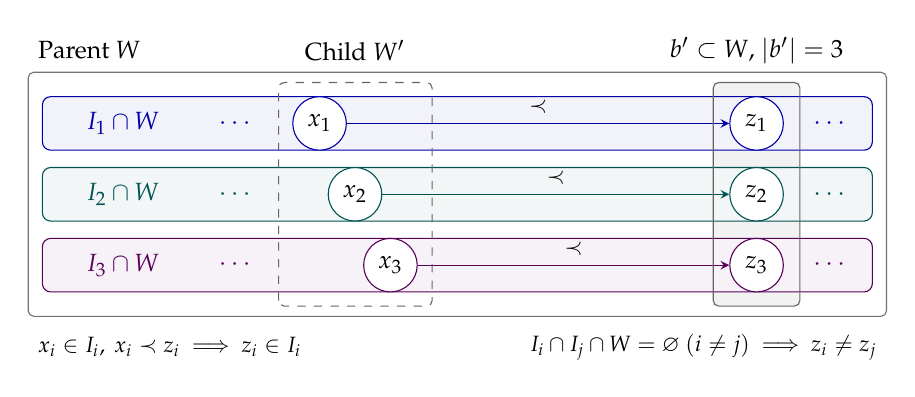
\begin{tikzpicture}[x=1cm,y=1cm,font=\small,>=stealth,
  job/.style={circle,draw,fill=white,minimum size=6.8mm,inner sep=0pt}]
  \draw[black!55,rounded corners=2pt] (-.15,-.25) rectangle (10.75,2.85);
  \node[anchor=west] at (-.15,3.13) {Parent $W$};
  \node at (4,3.13) {Child $W'$};
  \node at (9.1,3.13) {$b'\subset W$, $|b'|=3$};

  \fill[black!5] (8.55,-.12) rectangle (9.65,2.72);
  \foreach \yy/\ii/\xx/\cc in {2.2/1/3.55/blue!65!black,1.3/2/4/teal!65!black,.4/3/4.45/violet!70!black} {
    \draw[draw=\cc,fill=\cc!5,rounded corners=3pt]
      (.03,\yy-.34) rectangle (10.57,\yy+.34);
    \node[text=\cc] at (1.05,\yy) {$I_{\ii}\cap W$};
    \node[text=\cc] at (2.5,\yy) {$\cdots$};
    \node[job,draw=\cc] (x\ii) at (\xx,\yy) {$x_{\ii}$};
    \node[job,draw=\cc] (z\ii) at (9.1,\yy) {$z_{\ii}$};
    \draw[->,draw=\cc] (x\ii) -- node[above,font=\footnotesize] {$\prec$} (z\ii);
    \node[text=\cc] at (10.05,\yy) {$\cdots$};
  }
  \draw[dashed,black!60,rounded corners=2pt] (3.03,-.12) rectangle (4.98,2.72);
  \draw[black!60,rounded corners=2pt] (8.55,-.12) rectangle (9.65,2.72);
  \node[anchor=west,font=\footnotesize] at (-.15,-.64)
    {$x_i\in I_i,\ x_i\prec z_i\ \Longrightarrow\ z_i\in I_i$
     };
  \node[anchor=east,font=\footnotesize] at (10.75,-.64)
    {$I_i\cap I_j\cap W=\varnothing\ (i\ne j)\ \Longrightarrow\ z_i\ne z_j$};
\end{tikzpicture}

\caption{Why at most three injections survive a same-direction update.
For each surviving injection, choose a high job $x_i$ in the child
and a successor $z_i$ in its ending triple $b'$.
Upward closure puts $z_i$ in the same injection; disjointness on the
parent $W$ makes the chosen $z_i$ distinct.
The three-injection case is drawn; arrows denote precedence.
Only witness pairs are shown:
the injections may contain other jobs and may overlap outside $W$.}
\label{fig:capacity-three}
\end{figure}


\subsection{Flattening the history of a run}

Only the first entry of a switch pair can carry a complicated predicate
from an earlier run. The following lemma removes it whenever we need
to reconstruct an old cutoff on a descendant parent.

\begin{lemma}[Local flattening]\label{lem:flatten}
Suppose a run began with a switch out of a node \(Q_0\), using
left boundary \(a_0\) in the resulting run frame, and entries
\[
 G_0\cap\{\rk\ge h_0\},\qquad D_{a_0},
 \qquad Q_0\setminus D_{a_0}\subseteq G_0 .
\]
Let \(U\subseteq Q_0\) be a later parent in that run. If the entry derived from the first displayed entry
survives into an unpruned carry out of \(U\), write its
current form as \(G_0\cap\{\rk\ge k\}\). Then the carried portion
of this pair has the same union on \(U\) as the global upset
\begin{equation}
 D_{a_0}\cup\{\rk\ge k\}.
 \label{eq:flatten}
\end{equation}
\end{lemma}
\begin{proof}
Track the original entries through later reindexings.
As long as the first entry survives, a suffix operation cannot
trim or discard the second entry: a cutoff at that later index
would already discard the first, permanently.
Thus the second entry is either still carried untrimmed, or was
pruned because it was empty on some intermediate node containing
\(U\). In the latter case \(D_{a_0}\cap U=\varnothing\).

On \(U\cap D_{a_0}\), the second entry, when this set is nonempty,
therefore selects every job. Every job of
\(U\setminus D_{a_0}\) lies in \(G_0\), because \(U\subseteq Q_0\).
On that remainder the first entry selects exactly the rank suffix
\(\rk\ge k\). This proves equality of the two unions on \(U\).
Both factors in \eqref{eq:flatten} are upsets, so their union is
globally upward closed, although it need not agree with the
carried pair outside \(U\).
\end{proof}

A new switch out of a node \(W\) uses the edge \(U\to W\)
by which \(W\) was created. Let \(H_-\) be that incoming
edge's low cutoff, in its own working frame, and reserve \(S\)
for the cutoff of the new outgoing edge. We need an extension
of \(H_-\) that does not retain a complicated switch predicate
from an earlier run. Local flattening provides it using lists and
covering properties belonging to already constructed ancestors.

\begin{lemma}[A short extension of an earlier low set]\label{lem:old-low}
Consider an already constructed edge from a parent \(U\) to a child
\(W\), in its old working frame. Its low cutoff \(H_-\subseteq U\)
has a global downset extension \(H_-^*\) agreeing with it on \(U\).
This extension can be chosen with at most \(21\) leaves.
\end{lemma}
\begin{proof}
Use the boundary notation of \(U\) in that old frame for this proof.
If the edge was a switch relative to the tag of \(U\), its low
cutoff is a rank prefix of \(U\setminus D_a\). Thus
\[
 (J\setminus D_a)\cap\{\rk\le r\}
\]
is the required global downset, using at most two leaves.

If the edge was same, its low cutoff on \(U\) equals \(P_b\)
minus its unpruned carry union, without the fresh injection.
The old list on \(U\) has at most five entries by
\Cref{lem:list-length}. If its run began at the root, all carry
entries are simple: the root base or injections, possibly rank-trimmed.
If it began at a switch, the only possibly complicated carry
entry is the first of that switch pair. If it is present in the carry,
replace the carried pair by \eqref{eq:flatten}; if it is absent from
the carry, every carried entry is already simple.

This gives a global upset agreeing with the carry union on \(U\).
It has at most five terms, each with at most four leaves.
Indeed an injection with a rank trim has three leaves; a root
base or a second switch base with a trim has at most two; and
the flattened pair has two. Taking \(P_b\) minus this union
gives a global downset with at most \(1+5\cdot4=21\) leaves.
An empty carry is represented by false.
\end{proof}

\subsection{Constructing the new switch upset}

Suppose a switch out of \(W\) produces a nonempty child.
By \Cref{lem:edge-labels}, \(W\) is not the root.
Let \(U\) be the parent that produced \(W\).
That preceding edge was taken in the tag frame of \(W\), which
is opposite to the current working frame.
In the current frame write \(a_-,b_-\) for the boundaries of \(U\)
and \(v_-\) for its center. The temporal arrangement is
\begin{equation}
 a_-<v_-\le a<b\le b_-.
 \label{eq:ancestry}
\end{equation}
Here \(a\) is an actual ending endpoint of that preceding edge,
viewed in reverse; it can equal \(v_-\).
The node \(W\) lies in the open suffix of \(U\) after \(v_-\);
Figure~\ref{fig:switch} shows this arrangement.

Let \(H_-\) be the low set of the preceding edge in its old
working frame, regarded as a subset of all of \(U\).
The extension \(H_-^*\) from \Cref{lem:old-low} is an upset in
the current, reversed frame. Define
\begin{equation}
 G=D_{a_-}\cap(J\setminus\wP a)
            \cap(J\setminus\wP{v_-})\cap H_-^* .
 \label{eq:G}
\end{equation}

\Needspace{3\baselineskip}
\begin{lemma}\label{lem:G}
The set \(G\) in \eqref{eq:G} is a global upset satisfying both
properties in \eqref{eq:G-properties}.
\end{lemma}
\begin{proof}
All four factors in \eqref{eq:G} are global upsets in the current
frame, so \(G\) is an upset.

Let \(x\in X=W\setminus D_a\).
If \(x\) had been high at the preceding edge in its old frame,
\Cref{lem:edge-labels} would put it in the old predecessor cone
of that edge's ending endpoint. That endpoint is the current \(a\),
so reversal would give \(x\in D_a\), a contradiction.
Thus \(x\in H_-\).
Every job of \(H_-\) precedes the old right boundary of \(U\),
because all edge cutoffs lie in that cone. Equivalently,
\(H_-\subseteq D_{a_-}\) in the current frame.
Since \(x\) is strictly after both \(a\) and \(v_-\), feasibility
excludes \(x\) from their weak predecessor cones.
Finally, \(x\in U\), so agreement of \(H_-^*\) on \(U\) gives
\(x\in H_-^*\). Hence \(X\subseteq G\).

Conversely, suppose \(z\in G\) is scheduled at or before \(a\).
Membership in \(D_{a_-}\), together with \eqref{eq:ancestry},
first places it strictly inside \(U\):
\begin{equation}
 a_-<\operatorname{time}(z)\le a<b\le b_-.
 \label{eq:localize-U}
\end{equation}
Only now use \(H_-^*\cap U=H_-\).
The old edge cutoff \(H_-\) was contained in the old center-low
set. If \(z\) is at or before \(v_-\) in the current frame,
the old center separator puts it in current \(\wP{v_-}\).
If it is strictly after \(v_-\) but at or before \(a\), it lies
in the old normalized side and the old separator at the endpoint
\(a\) puts it in current \(\wP a\).
Both possibilities contradict \eqref{eq:G}.

These separator implications remain valid when preparing the current
node: all intervening reorderings have been confined to \(W=(a,b)\),
and therefore have not changed any job at or before \(a\) in the
current frame, the relevant boundary triples, or the fixed old
cutoff sets.
\end{proof}

\begin{figure}[t]
\centering
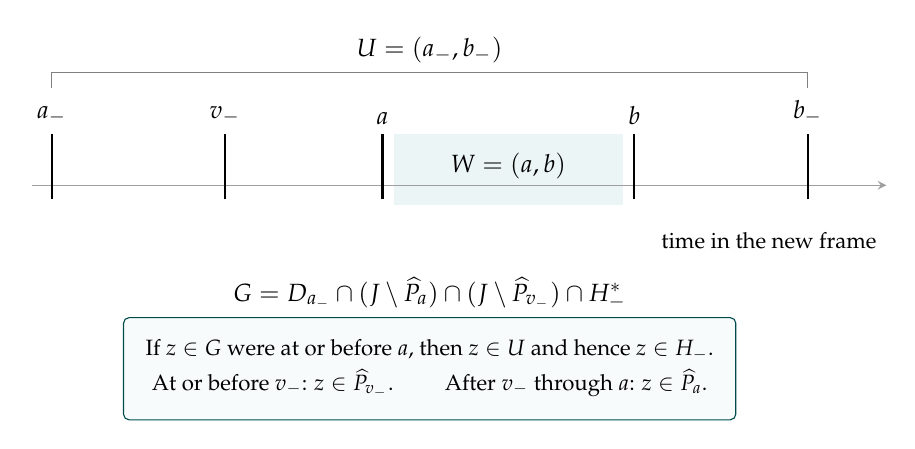
\begin{tikzpicture}[x=1cm,y=1cm,font=\small,>=stealth]
  \fill[teal!8] (4.35,-.25) rectangle (7.25,.65);
  \draw[->,gray!75] (-.25,0) -- (10.6,0);
  \foreach \x in {0,2.2,4.2,7.4,9.6}
    {\draw[thick] (\x,-.18) -- (\x,.65);}
  \node[above] at (0,.65) {$a_-$};
  \node[above] at (2.2,.65) {$v_-$};
  \node[above] at (4.2,.65) {$a$};
  \node[above] at (7.4,.65) {$b$};
  \node[above] at (9.6,.65) {$b_-$};
  \node at (5.8,.25) {$W=(a,b)$};
  \draw[gray] (0,1.24) -- (0,1.43) -- (9.6,1.43) -- (9.6,1.24);
  \node[above] at (4.8,1.43) {$U=(a_-,b_-)$};
  \node[anchor=east,font=\footnotesize] at (10.6,-.7)
    {time in the new frame};
  \node[anchor=north,align=center] at (4.8,-1.05)
    {$G=D_{a_-}\cap (J\setminus\widehat P_a)
      \cap (J\setminus\widehat P_{v_-})\cap H_-^*$};
  \node[draw=teal!60!black,fill=teal!3,rounded corners=2pt,
        inner sep=8pt,align=center,font=\footnotesize] at (4.8,-2.33)
    {If $z\in G$ were at or before $a$, then $z\in U$ and hence $z\in H_-$.\\[3pt]
     At or before $v_-$: $z\in\widehat P_{v_-}$.
     \qquad After $v_-$ through $a$: $z\in\widehat P_a$.};
\end{tikzpicture}

\caption{The ancestor configuration at a direction change, in the new
working frame. A candidate early member of \(G\) is first located
inside \(U\) by \(D_{a_-}\); only there is the earlier cutoff
extension used. The two weak predecessor exclusions then cover
the portions at or before \(v_-\) and between \(v_-\) and \(a\).
The equality \(a=v_-\) is allowed; the intervening segment then
collapses. The horizontal arrow denotes time.}
\label{fig:switch}
\end{figure}

\subsection{Predicate bounds and the induction order}

\begin{lemma}\label{lem:entry-size}
Every entry constructed above has fewer than \(40\) leaves.
This bound persists through any number of same-direction updates.
\end{lemma}
\begin{proof}
Root bases, injections, and second switch bases are simple predicates.
By \Cref{lem:old-low}, the \(H_-^*\) factor in a new \(G\)
has at most \(21\) leaves. The three other factors of \(G\)
and its outer rank suffix use four more. Thus a new first switch
entry has at most \(25\) leaves.
Further same-direction trimming only tightens that outer rank
suffix. It does not append a new independent condition.
The same observation applies to simple entries.
\end{proof}

For completeness, the construction so far has a well-founded
dependency order. Assume the parent and ancestor data already satisfy
their assertions. A same update is defined directly. A switch update
uses the preceding edge's low set; \Cref{lem:old-low} derives its
short extension from already existing lists and, when necessary,
an earlier switch's covering property. \Cref{lem:G} then proves
the new covering and early-exclusion properties.
\Cref{lem:update-labels} supplies the high-set identity and
Invariant~\ref{inv:cones}; \Cref{lem:list-length} supplies the new
length bound; and \Cref{lem:entry-size} supplies the predicate bound.
The length argument needs global closure and high-set identities,
but not the numerical predicate bound. Thus neither bound assumes
itself at a deeper node.

The root starts this induction. We next prove the remaining boundary
invariants for every update, using only the parent invariants and
the current normalizations.

\section{Preserving the global boundary invariants}\label{sec:boundary}

We verify Invariants~\ref{inv:past} and~\ref{inv:swap}
for a child \(W'=(a',b')\) of \(W=(a,b)\).
All notation is in the working frame of the child edge.
In a same update this is also the parent's tag frame.
In a switch update the old list is not carried; the newly constructed
upsets are used instead.

Preparatory changes to the schedule of \(W\) preserve the parent
invariants. Its boundary triples and all earlier exterior jobs
stay fixed, so Invariant~\ref{inv:past} is unchanged.
Invariant~\ref{inv:swap} already quantifies over every feasible
reordering of \(W\).

\subsection{Excluding distant qualifiers}

\begin{lemma}\label{lem:past}
The updated child list satisfies Invariant~\ref{inv:past}.
\end{lemma}
\begin{proof}
It suffices to prove the assertion before pruning, since pruning only
removes qualifiers. Let \(z\) qualify for the pre-pruning child list and be scheduled
at or before \(a'\).

If \(a<\operatorname{time}(z)\le a'\), the job belongs to the normalized
open side \(E\) of the parent. By \Cref{lem:update-labels}, it is
high at the edge cutoff \(S\). The local separator at \(a'\) puts
it in \(P_{a'}\) when strictly earlier, and membership in the
triple puts it in \(\wP{a'}\) when its time equals \(a'\).

Now suppose \(z\) is at or before \(a\).
The new injection \(D_a\setminus P_b\) cannot contain such a job.
Nor can either switch entry, by \Cref{lem:G} and the strictness
of \(D_a\). Thus the only remaining case is a same-direction
carry qualifier.
The parent's Invariant~\ref{inv:past} supplies a job \(y\in a\)
with \(z=y\) or \(z\prec y\).
The carry is a global upset, so \(y\) also qualifies by carry.
In particular \(a\) is actual. If \(a'=a\), we are done.

Assume \(a'>a\), and write \(a'=s_i\), with edge cutoff \(S=S_i\).
Follow all the strict advances of the walk from \(a\) through
promotion \(i\), including intermediate advances not retained as marks.
Every cutoff used in this portion of the walk is contained in \(S_i\).
On \(W\), the final carry is exactly \(O\setminus S_i\).
Consequently every carry qualifier in \(E\) is high, and has worse
priority than the low exceptions, at every one of these advances.

The first advance needs the parent exchange invariant, because
\(a\) lies outside the normalized open side \(E\).
Consider that first actual advance off \(a\), with earliest exception
\(x\) at its target \(t\).
All \emph{global} predecessors of \(x\) are before \(a\).
To verify this stronger readiness assertion, every predecessor is
temporally before \(t\). If one were at \(a\), then \(x\in D_a\).
If one were strictly between \(a\) and \(t\), it would belong to
the contiguous side \(E\), be low, and descend from \(a\) by
earliestness of the exception. Again \(x\in D_a\), a contradiction.
There is no other possible predecessor at or after \(a\).

Also \(x\in X=W\setminus D_a\), so Invariant~\ref{inv:cones}
puts it among the old qualifiers, outside the starting low set.
It has already been promoted by stage \(i\), so its old key is
strictly below the least unpromoted key at \(S_i\).
By \Cref{lem:carry}, the boundary job \(y\) has old key at least
that least unpromoted key.
The parent's Invariant~\ref{inv:swap}, applied after the current
preparatory reorderings of \(W\), therefore prohibits exchanging
\(x\) and \(y\) in the complete schedule.

If \(y\) had no global successor at or before \(t\), that exchange
would be feasible. All global predecessors of \(x\) lie strictly before \(a\);
moving it earlier preserves its successor constraints, and delaying
\(y\) to \(t\) preserves its predecessor constraints and, under
the supposition, its successor constraints. Thus \(y\) must have
a strict successor by \(t\).
Such a successor is in \(E\) and is still a carry qualifier.

Any carry job strictly between \(a\) and \(t\) must likewise have
a successor by \(t\): otherwise exchange it with \(x\) within
\(E\), contradicting its lexicographic normalization.
The carry is an upset, so these successors remain in the carry.
Iterating along strictly increasing times reaches a carry job
at \(t\). It cannot be \(x\), which is low and lies outside
the final carry.

At every subsequent advance, the local readiness and exchange argument
from \Cref{lem:shared} applies inside \(E\). All carry jobs remain
high at that advance, so each carry job at its starting slot
has a carry descendant at its target. Tracing from the descendant
of \(y\) at the first target eventually gives a descendant of
\(y\) at \(a'\).
Hence \(z\in\wP{a'}\), as required.
\end{proof}

\subsection{Exchanges after future child reorderings}

\begin{lemma}\label{lem:swap}
The pruned child list satisfies Invariant~\ref{inv:swap},
with its quantifier over all feasible reorderings of \(W'\).
\end{lemma}
\begin{proof}
Take any feasible reordering of \(W'\) in its slots.
Suppose \(x\in W'\setminus D_{a'}\), that \(y\in a'\)
qualifies for the child list, and that the new key of \(x\)
is smaller than the new key of \(y\).
Invariant~\ref{inv:cones}, already proved for the child in
\Cref{lem:update-labels}, ensures that \(x\) qualifies.
By \Cref{lem:prune}, the same comparison holds in the new list
before pruning.

First let \(a'>a\). Both \(x\) and \(y\) are in the parent's
normalized side \(E\), and both are high at its edge cutoff \(S\),
by \Cref{lem:update-labels}. The pre-pruning key order agrees with
the priority order used to normalize \(E\). Thus \(x\) has
better priority than \(y\).
The child reordering changes only slots strictly after \(a'\).
A feasible exchange of \(x,y\) in the complete schedule would
therefore give a feasible full schedule of the same \(E\)
with a better prefix at \(a'\), contrary to
\Cref{lem:lex-prefix}.

Now let \(a'=a\).
In the switch case there is no new qualifier at \(a\), so no
such \(y\) exists.
In the same case neither \(x\) nor \(y\) belongs to the new
injection: \(x\notin D_a\), and no job at \(a\) is a strict
descendant of \(a\).
Their pre-pruning comparison therefore uses only carry entries.
By \Cref{lem:carry}, it implies the same old key comparison
in the parent's list.
Moreover \(x\in W\setminus D_a\).
The preparatory reorderings and the arbitrary subsequent reordering
of \(W'\) together form a feasible reordering confined to \(W\).
The parent's Invariant~\ref{inv:swap} rules out the proposed
exchange.
\end{proof}

\begin{proposition}\label{prop:construction-valid}
Starting from any feasible full schedule, the marking and list
construction is defined at every node. Its pruned lists are global
upset lists of length at most five, with fewer than \(40\) leaves
per entry, and satisfy Invariants~\ref{inv:cones}--\ref{inv:swap}.
Every branch terminates.
\end{proposition}
\begin{proof}
Proceed by depth from the root data of \Cref{sec:construction}.
Given valid ancestor and parent data, the center and the two
normalized sides exist by \Cref{cor:any-ideal,lem:reorder}.
The shared walk and \Cref{lem:edge-labels} define the children.
For a same update the new list is direct. For a switch,
\Cref{lem:old-low,lem:G} construct the needed global upset
using only earlier data, as explained at the end of
\Cref{sec:lists}.
Then \Cref{lem:update-labels,lem:list-length,lem:entry-size}
give the first invariant and the bounds.
\Cref{lem:past,lem:swap} give the other two invariants without
using a claim about any deeper child.
This completes the simultaneous induction.
Every child omits the center, so its size decreases strictly.
\end{proof}

Invariant~\ref{inv:past} will let a bounded predicate distinguish
the child from qualifiers arbitrarily far in the past.
Invariant~\ref{inv:swap} is what allows that first invariant to
continue propagating after recursive reorderings. Neither is
replaced by an assertion only about local separators.

\section{Global interval predicates and completion}\label{sec:descriptions}

We now describe each child as a global set without intersecting
with a recursively described parent. This is the step that converts
the construction into a polynomial family of subproblems.

\subsection{Global tests for local cutoffs}

The cutoff predicates in this section are used only in the final
interval and split formulas. The list construction and its entry-size
bound are now complete, so these formulas may retain the existing
bounded entries. The historical extension in \Cref{lem:old-low},
by contrast, had to flatten an earlier run before a new switch
entry could be constructed.

For every walk cutoff \(S\) in a parent \(W\), choose a global
predicate \(\widetilde S\) satisfying
\begin{equation}
 \widetilde S\cap W=S.
 \label{eq:cutoff-agreement}
\end{equation}
In the same case, let \(\K_{\mathrm{carry}}\) be the carry determined
by \(O\setminus S\), before the new injection. Use
\begin{equation}
 \widetilde S=P_b\setminus\Qual(\K_{\mathrm{carry}}).
 \label{eq:direct-same-cutoff}
\end{equation}
On \(W\), the carry selects precisely \(O\setminus S\), while
the low jobs are the initial \((W\setminus O)\cap P_b\) and the
promoted portion of \(O\). Thus \eqref{eq:cutoff-agreement} holds.
In the switch case use
\begin{equation}
 \widetilde S=(J\setminus D_a)\cap\{\rk\le r\},
 \label{eq:direct-switch-cutoff}
\end{equation}
where \(r\) is the rank of the last promoted member of \(X\),
or \(r=0\) before any promotion.
These formulas are available at every walk cutoff, whether or not
the associated open gap is nonempty.
They are not required to have any prescribed meaning outside \(W\).

\subsection{A child as a global set}

Figure~\ref{fig:gap} summarizes the localization steps in the following
formulas.

\begin{lemma}\label{lem:global-child}
In the valid construction of \Cref{prop:construction-valid}, let
\(W'=(a',b')\) be a child of \(W=(a,b)\), with parent center \(v\),
edge cutoff \(S\), new pruned list \(\K'\), and cutoff predicate
\(\widetilde S\) satisfying \eqref{eq:cutoff-agreement}.
In the edge's working frame, its high and low parts are the
following global sets:
\begin{align}
 W'\setminus S
 &=\Qual(\K')\cap P_{b'}\cap(J\setminus\wP{a'}),
 \label{eq:global-high}\\
 W'\cap S
 &=D_{a'}\cap P_b\cap(J\setminus\wD{b'})
                  \cap(J\setminus\wD v)\cap\widetilde S .
 \label{eq:global-low}
\end{align}
\end{lemma}
\begin{proof}
Every high child job qualifies, precedes \(b'\), and, because
it is later than \(a'\), is outside \(\wP{a'}\).
Conversely, a job selected by the right side of
\eqref{eq:global-high} is strictly before \(b'\) by precedence.
If it were at or before \(a'\), the child's global
Invariant~\ref{inv:past} would put it in \(\wP{a'}\).
It is therefore strictly in \(W'\), and the child list selects
exactly its high jobs.

For \eqref{eq:global-low}, consider first a job selected by its
right side. The two positive tests \(D_{a'}\cap P_b\) locate
it strictly inside the parent \(W\): its time is after
\(a'\ge a\) and before \(b\). This remains true with sentinel
boundaries under our conventions.
We can consequently use \eqref{eq:cutoff-agreement} to infer
that the job is in \(S\).
This cutoff is contained in the center-low set \(S_*\).
A selected job at or after \(v\) would therefore lie in
\(\wD v\), by the center separator or by membership in \(v\)
itself. The corresponding exclusion places it in the open side
\(E=(a,v)\).
Within \(E\), a low job at or after \(b'\) is in
\(\wD{b'}\), using the local separator at \(b'\).
The remaining exclusion puts the selected job strictly between
\(a'\) and \(b'\).

Conversely, a low job of this gap lies in \(D_{a'}\cap P_b\)
by \Cref{lem:edge-labels}, and it satisfies
\(\widetilde S\) by \eqref{eq:cutoff-agreement}.
Its time is strictly before both \(b'\) and \(v\), so it is
in neither of their weak successor cones. It passes every test
in \eqref{eq:global-low}.
\end{proof}

\begin{figure}[t]
\centering
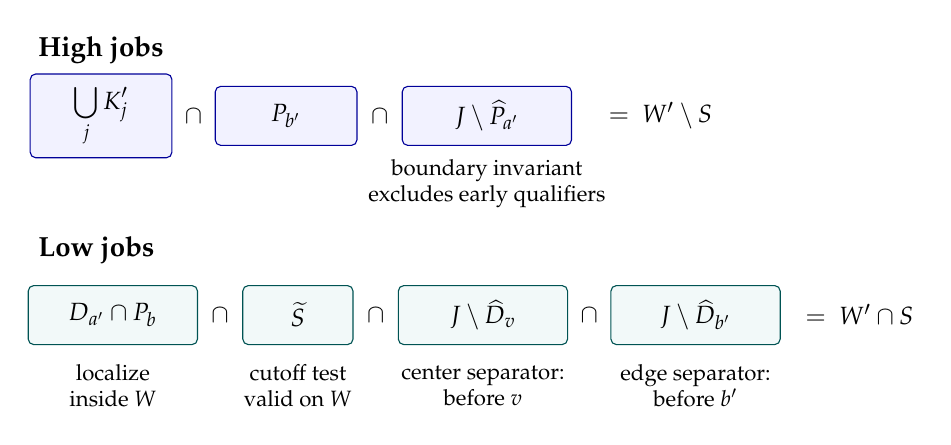
\begin{tikzpicture}[x=1cm,y=1cm,font=\small,
  filter/.style={draw,rounded corners=2pt,minimum height=.75cm,
                 minimum width=1.8cm,inner sep=4pt,align=center}]
  \node[anchor=west,font=\bfseries] at (-.92,2.18) {High jobs};
  \node[filter,draw=blue!60!black,fill=blue!5] (h1) at (0,1.35)
    {$\displaystyle\bigcup_j K'_j$};
  \node[filter,draw=blue!60!black,fill=blue!5] (h2) at (2.35,1.35)
    {$P_{b'}$};
  \node[filter,draw=blue!60!black,fill=blue!5,minimum width=2.15cm] (h3) at (4.9,1.35)
    {$J\setminus\widehat P_{a'}$};
  \node at (1.175,1.35) {$\cap$};
  \node at (3.54,1.35) {$\cap$};
  \node[anchor=west] at (6.32,1.35) {$=\ W'\setminus S$};
  \node[font=\footnotesize,align=center] at (4.9,.49)
    {boundary invariant\\excludes early qualifiers};

  \node[anchor=west,font=\bfseries] at (-.92,-.36) {Low jobs};
  \node[filter,draw=teal!65!black,fill=teal!5,minimum width=2.15cm] (l1) at (.15,-1.18)
    {$D_{a'}\cap P_b$};
  \node[filter,draw=teal!65!black,fill=teal!5,minimum width=1.4cm] (l2) at (2.5,-1.18)
    {$\widetilde S$};
  \node[filter,draw=teal!65!black,fill=teal!5,minimum width=2.15cm] (l3) at (4.85,-1.18)
    {$J\setminus\widehat D_v$};
  \node[filter,draw=teal!65!black,fill=teal!5,minimum width=2.15cm] (l4) at (7.55,-1.18)
    {$J\setminus\widehat D_{b'}$};
  \node at (1.51,-1.18) {$\cap$};
  \node at (3.49,-1.18) {$\cap$};
  \node at (6.20,-1.18) {$\cap$};
  \node[anchor=west] at (8.82,-1.18) {$=\ W'\cap S$};
  \node[font=\footnotesize,align=center] at (.15,-2.08)
    {localize\\inside $W$};
  \node[font=\footnotesize,align=center] at (2.5,-2.08)
    {cutoff test\\valid on $W$};
  \node[font=\footnotesize,align=center] at (4.85,-2.08)
    {center separator:\\before $v$};
  \node[font=\footnotesize,align=center] at (7.55,-2.08)
    {edge separator:\\before $b'$};
\end{tikzpicture}

\caption{The two global tests for a child.
For the low part, positive cones locate a candidate inside the parent
before its cutoff predicate is used; the two weak successor exclusions
then restrict that candidate to the gap.
For the high part, the global past-boundary invariant excludes
qualifiers at or before \(a'\).
The intersection factors are arranged in the order used by the proof.}
\label{fig:gap}
\end{figure}

The localization order matters. Neither the cutoff extension
\(\widetilde S\) nor the flattened historical extension needs to
agree with its intended local set everywhere in \(J\).
Positive cone tests first place the candidate in the domain where
agreement is known. The construction never appends a membership
predicate for all ancestor intervals.

\subsection{Relative predicates for the marked splits}

\begin{lemma}\label{lem:relative-splits}
Every marked slot \(z\) in a node \(W\) has a bounded relative
description of its earlier jobs in either the working direction
that produced it or the original direction. The formulas use the stated
atomic language and have fewer than \(500\) leaves, as counted in
\Cref{lem:final-count}.
\end{lemma}
\begin{proof}
Use the working frame for a side, and put
\[
 H_*=
 \begin{cases}
 P_b,&\same,\\
 J\setminus D_a,&\switch.
 \end{cases}
\]
For the center \(v\), the predicate \(B_v(H_*)\), restricted to
\(W\), is its earlier set, by
\Cref{lem:separator-description} and \eqref{eq:center-cutoff}.

For an internal mark \(z\) in the open side \(E\), choose a walk
cutoff \(S\) for which it is a local separator.
The predicate
\begin{equation}
 F_z=B_v(H_*)\cap B_z(\widetilde S)
 \label{eq:relative-split}
\end{equation}
gives its earlier set upon restriction to \(W\).
The first factor selects \(E\) on \(W\); on that domain the
second is the separator description from
\Cref{lem:separator-description}.

If the working frame is opposite to original time, \(F_z\cap W\)
describes the original \emph{later} jobs. Replace \(F_z\) by
\begin{equation}
 (J\setminus F_z)\setminus z
 \label{eq:reverse-split}
\end{equation}
to obtain the original earlier jobs after restriction to \(W\).
The exclusion of the marked triple is necessary: complementation
alone includes it. Apply the same conversion to the center
predicate when appropriate.
\end{proof}

\begin{lemma}\label{lem:final-count}
The predicates in \Cref{lem:global-child,lem:relative-splits}
have fewer than \(500\) leaves.
\end{lemma}
\begin{proof}
A pruned list or a carry contains at most five entries with fewer
than \(40\) leaves each, so its union has at most \(195\) leaves.
An empty union uses the false constant.
The same-direction cutoff \eqref{eq:direct-same-cutoff} therefore
needs at most \(196\) leaves; the switched one needs two.
Use \(205\) as a common loose allowance.

The high predicate \eqref{eq:global-high} uses at most
\(195+2=197\) leaves. The low predicate
\eqref{eq:global-low} uses at most \(205+4=209\).
Their union is a global description of \(W'\) with at most
\(406\) leaves.

The center predicate has three leaves. The internal split
\eqref{eq:relative-split} has at most \(3+(205+2)=210\),
and conversion \eqref{eq:reverse-split} adds one.
Complementation does not increase leaf counts.
Every cone uses an actual triple or a sentinel constant; all ranks
and thresholds are from the two allowed frames. Thus these are
formulas in the stated atomic language.
\end{proof}

\begin{proof}[Proof of \Cref{thm:structure}]
Use \Cref{prop:construction-valid} to construct marks and lists
from a feasible full schedule.
The root set \(J\) is represented by true.
Every nonempty child has the global description supplied by
\Cref{lem:global-child}. Every mark has the relative split
description supplied by \Cref{lem:relative-splits}.
\Cref{lem:final-count} places both kinds of description in
\(\F\), independently of their depth.
All branches terminate because the node sizes decrease strictly.
These are exactly the conditions of \Cref{def:hierarchy}.
\end{proof}

\section{Running time in the explicit input model}\label{sec:complexity}

The preceding structural proof establishes completeness of the finite
search. We now give the detailed deterministic multitape accounting
promised in \Cref{prop:algorithm}. Its purpose is to make the
polynomial-time assertion uniform; the structural argument does not
require efficient normalization of a schedule or a small recursion depth.

\begin{proof}[Running-time bound in \Cref{prop:algorithm}]
First specify a conservative implementation using sequential scans.
Write \(B=C_KN^{3K}\) for an upper bound on the number of enumerated
formulas, where \(C_K\) depends only on the fixed \(K\).
There are at most \(B\) distinct sets and at most \(S=BN^3\)
candidate states for each \(W\).
Store their bit vectors, reachability marks, and predecessor record
numbers on work tapes. Each state record uses \(O_K(N)\) bits:
its indices require only \(O_K(\log N)\) bits.
Store an explicit full schedule with each previously accepted set.
This table uses \(O_K(BN^2)\) bits, since a schedule lists at most
\(N\) job identifiers and their slots.

A complete scan to fetch or update a state record costs
\(O_K(SN)=O_K(BN^4)\) steps. A lookup in the acceptance table by
comparing all bit vectors costs \(O_K(BN^2)\) steps.
Even checking all required precedence relations by repeated scans of
the \(N\)-by-\(N\) reachability table costs at most \(O(N^4)\).
Thus one ordered state-pair test and reachability update costs
\(O_K(BN^4)\) steps, without constant-time random access.
Starting from the initial states, make at most \(S\) passes over all
ordered pairs, marking a target when its source is marked and
\eqref{eq:transition} holds. These passes find every reachable state.
For all sets together their cost is at most
\[
 O_K\bigl(BS^3BN^4\bigr)
 =O_K(B^5N^{13})
 =O_K(N^{15K+13}).
\]
Generating, evaluating, and deduplicating formulas by scans costs at
most \(O_K(B^2N^4)\); reachability preprocessing, state construction,
and table initialization also fit within the displayed bound.
The subscript \(K\) denotes a constant fixed independently of the input.
Since \(N\le3n\) and the vertices are explicitly listed, the looser
bound \(O((L+2)^{150020})\) covers input processing and even all
\(n\) deadline trials needed for optimization.
\end{proof}

\begin{remark}\label{rem:compact}
For the deadline feasibility decision, the same preprocessing can handle
an encoding that specifies an enormous number of isolated vertices only
through a binary value of \(n\).
After checking \(n\le3T\), let \(d\) be the number of vertices appearing
in edges. If \(T\ge d\), accept: schedule those \(d\) vertices sequentially
in topological order and fill free positions with the isolated vertices.
Otherwise \(N=3T<3d\le6|E|\), so expansion is polynomial. This extra
branch is not needed for the explicit encoding in \Cref{thm:main}.
\end{remark}

\section{Conclusion}\label{sec:conclusion}

The finite search succeeds because every interval in a suitable recursive
schedule decomposition has a global description of bounded size,
independent of its depth. Local separator descriptions alone do not give
that guarantee: the short upset lists, the exterior boundary invariants,
and the simplification at direction changes prevent the accumulation of
ancestor information.

The resulting algorithm constructs an exact optimum for the stated
three-machine model. The fixed leaf allowance $10000$ and the explicit
large exponent establish polynomial time for the stated model.
The proof supplies no practical performance guarantee.


\bibliographystyle{plainnat}
\bibliography{references}
\end{document}
